% The scene of the survey how-to (docs/how-to/sonar-survey.md), world gz_sonar/worlds/sonar_survey.sdf.
% World frame: x forward, y to port, z up, meters. Surface z = 0; seabed
%   z(x,y) = -8 + 0.6 sin(2 pi x/25) cos(2 pi y/40) + 0.3 sin(2 pi (x+y)/13).
% BlueBoat on the surface (hulls at y = +-0.36), running along +x on y = 0 from x = -15.
% Sidescan (Omniscan 450 SS) at z = -0.08: a beam to each side, axis 15 deg down, 50 deg across track (-3 dB:
% 10 deg above to 40 deg below horizontal), 0.5 deg along track, range 30 m. The upper edge meets the surface at once;
% the lower edge meets the seabed about 9.5 m out, leaving the nadir gap; the 30 m range meets it about 28.9 m out.
% Profiler (Surveyor 240-16) at z = -0.08, looking down, 80 deg across track: about +-6.7 m on 8 m of water.
% Targets: steel drum 0.58 m dia x 0.88 m, across the track, at (10, 0); concrete block 0.5 m cube, yaw 0.3, at
% (20, 12); glass float r 0.2 at (30, -10).
% (a) section across the track at x = 20, looking forward, port on the left; (b) plan view, forward up, starboard
% right. True scale in both.
% Build: pdflatex sonar_survey_scene.tex, then pdftocairo to ../../how-to/images/sonar-survey-scene.{png,svg}
\documentclass[tikz,border=6pt]{standalone}
\usetikzlibrary{arrows.meta,calc}
\renewcommand{\familydefault}{\sfdefault}
\tikzset{
  lbl/.style={font=\sffamily\small},
  beam/.style={fill=black!7,draw=black,thin},
  dim/.style={thin,{Latex[length=1.6mm]}-{Latex[length=1.6mm]}},
  lead/.style={thin,black!70},
  declare function={
    zsb(\p,\q)=-8+0.6*sin(14.4*\p)*cos(9*\q)+0.3*sin(27.692*(\p+\q));   % degrees: 360/25, 360/40, 360/13
  },
}

\begin{document}
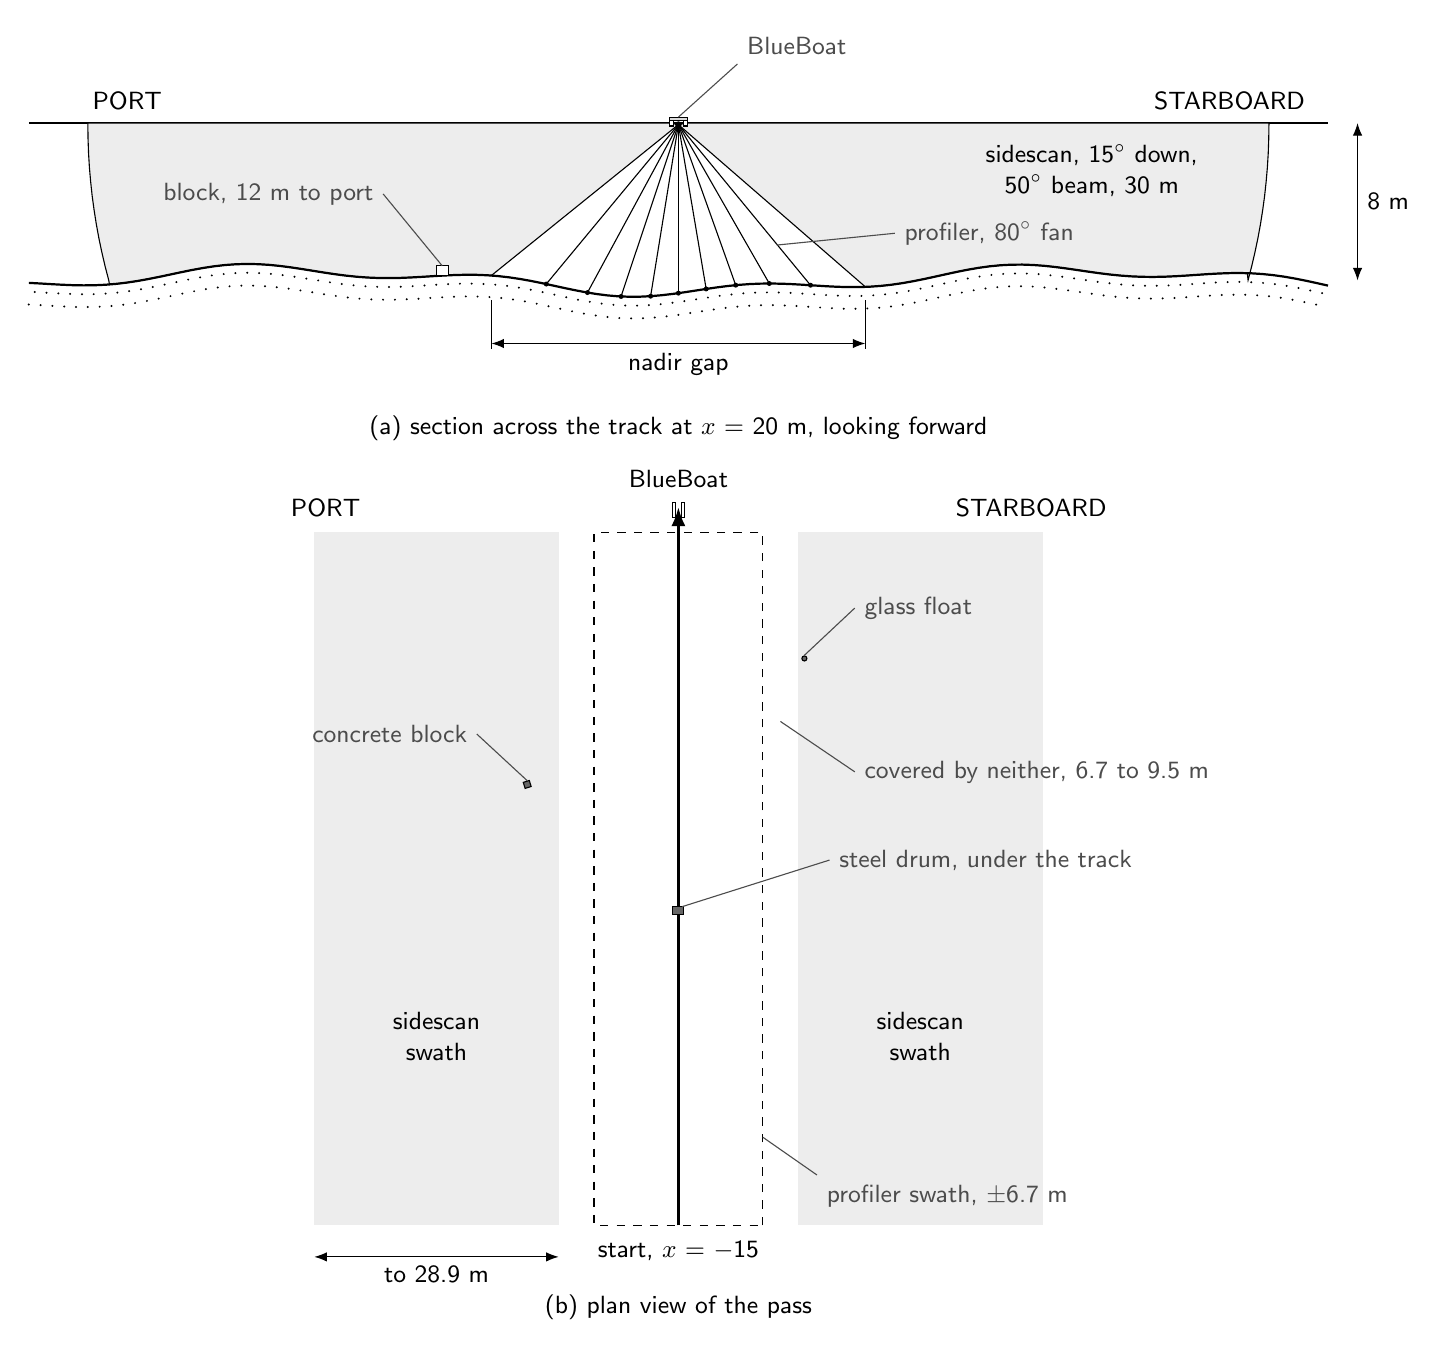
\begin{tikzpicture}
  % ================================================ (a) section at x = 20, looking forward: (y, z), port left
  \begin{scope}[x={(-0.25cm,0cm)},y={(0cm,0.25cm)}]
    \def\X{20}
    \pgfmathsetmacro{\af}{asin(7.9/30)}
    \draw[thin] (33,0) -- (-33,0);
    % sidescan beams, one per side: surface, 30 m range, seabed, lower edge
    % (the seabed runs 28.9 back to 9.5 as 38.4 - t)
    \draw[beam] (0,-0.08) -- (0.45,0) -- (30,0)
      -- plot[domain=0:\af,samples=12] ({30*cos(\x)},{-0.08-30*sin(\x)})
      -- plot[domain=9.5:28.9,samples=30] ({38.4-\x},{zsb(\X,38.4-\x)}) -- cycle;
    \draw[beam] (0,-0.08) -- (-0.45,0) -- (-30,0)
      -- plot[domain=0:\af,samples=12] ({-30*cos(\x)},{-0.08-30*sin(\x)})
      -- plot[domain=9.5:28.9,samples=30] ({\x-38.4},{zsb(\X,\x-38.4)}) -- cycle;
    % profiler fan, 80 deg across track
    \foreach \t in {-40,-30,...,40} {
      \pgfmathsetmacro{\yy}{8*tan(\t)}
      \draw[thin] (0,-0.08) -- (\yy,{zsb(\X,\yy)});
      \fill (\yy,{zsb(\X,\yy)}) circle (0.9pt);
    }
    % seabed, with two rows of dots below it
    \draw[thick] plot[domain=-33:33,samples=120] (\x,{zsb(\X,\x)});
    \foreach \r in {0.45,1.1} \foreach \k in {0,...,109}
      \fill ({-32.7+\k*0.6+0.3*mod(round(\r*10),2)},{zsb(\X,-32.7+\k*0.6+0.3*mod(round(\r*10),2))-\r}) circle (0.4pt);
    % concrete block at y = 12
    \draw[fill=white] (11.69,{zsb(\X,12)}) rectangle (12.31,{zsb(\X,12)+0.5});
    % boat: two hulls and a deck
    \draw[fill=white] (0.46,-0.15) rectangle (0.26,0.15) (-0.26,-0.15) rectangle (-0.46,0.15);
    \draw[fill=black!15] (0.46,0.15) rectangle (-0.46,0.3);
    \fill (0,-0.08) circle (1.2pt);
    % labels
    \node[lbl,anchor=south] at (28,0.2) {PORT};
    \node[lbl,anchor=south] at (-28,0.2) {STARBOARD};
    \draw[lead] (0,0.3) -- (-3,3) node[lbl,anchor=south west] {BlueBoat};
    \node[lbl,align=center] at (-21,-2.4) {sidescan, 15$^\circ$ down,\\50$^\circ$ beam, 30 m};
    \draw[dim] (-34.5,0) -- (-34.5,-8) node[lbl,midway,right] {8 m};
    \draw[dim] (9.5,-11.2) -- (-9.5,-11.2) node[lbl,midway,below] {nadir gap};
    \draw (9.5,-9) -- (9.5,-11.5) (-9.5,-9) -- (-9.5,-11.5);
    \draw[lead] (-5,-6.2) -- (-11,-5.6) node[lbl,anchor=west] {profiler, 80$^\circ$ fan};
    \draw[lead] (12,{zsb(\X,12)+0.5}) -- (15,-3.6) node[lbl,anchor=east] {block, 12 m to port};
    \node[lbl] at (0,-15.5) {(a) section across the track at $x$ = 20 m, looking forward};
  \end{scope}

  % ================================================ (b) plan view: forward up, starboard right
  \begin{scope}[shift={(0,-11.6)},x={(0cm,0.16cm)},y={(-0.16cm,0cm)}]
    \fill[black!7] (-15,9.5) rectangle (40,28.9);
    \fill[black!7] (-15,-9.5) rectangle (40,-28.9);
    \draw[dashed] (-15,-6.7) rectangle (40,6.7);
    \draw[thick,-{Latex[length=2.4mm]}] (-15,0) -- (42,0);
    % targets at true size
    \draw[fill=black!60] (9.71,-0.44) rectangle (10.29,0.44);
    \draw[fill=black!60,rotate around={17.2:(20,12)}] (19.75,11.75) rectangle (20.25,12.25);
    \draw[fill=black!60] (30,-10) circle (0.2);
    % boat at the end of the pass
    \draw[fill=white] (41.2,0.26) rectangle (42.4,0.46) (41.2,-0.46) rectangle (42.4,-0.26);
    % labels
    \draw[lead] (10.3,-0.3) -- (14,-12) node[lbl,anchor=west] {steel drum, under the track};
    \draw[lead] (20.3,12) -- (24,16) node[lbl,anchor=east] {concrete block};
    \draw[lead] (30.25,-10) -- (34,-14) node[lbl,anchor=west] {glass float};
    \node[lbl,anchor=north] at (-15.5,0) {start, $x$ = $-$15};
    \node[lbl,anchor=south] at (42.8,0) {BlueBoat};
    \node[lbl,align=center] at (0,19.2) {sidescan\\swath};
    \node[lbl,align=center] at (0,-19.2) {sidescan\\swath};
    \draw[lead] (-8,-6.7) -- (-11,-11) node[lbl,anchor=north west] {profiler swath, $\pm$6.7 m};
    \draw[lead] (25,-8.1) -- (21,-14) node[lbl,anchor=west] {covered by neither, 6.7 to 9.5 m};
    \node[lbl,anchor=south] at (40.5,28) {PORT};
    \node[lbl,anchor=south] at (40.5,-28) {STARBOARD};
    \draw[dim] (-17.5,9.5) -- (-17.5,28.9) node[lbl,midway,below] {to 28.9 m};
    \node[lbl] at (-21.5,0) {(b) plan view of the pass};
  \end{scope}
\end{tikzpicture}
\end{document}
